\begin{figure}
    \centering
    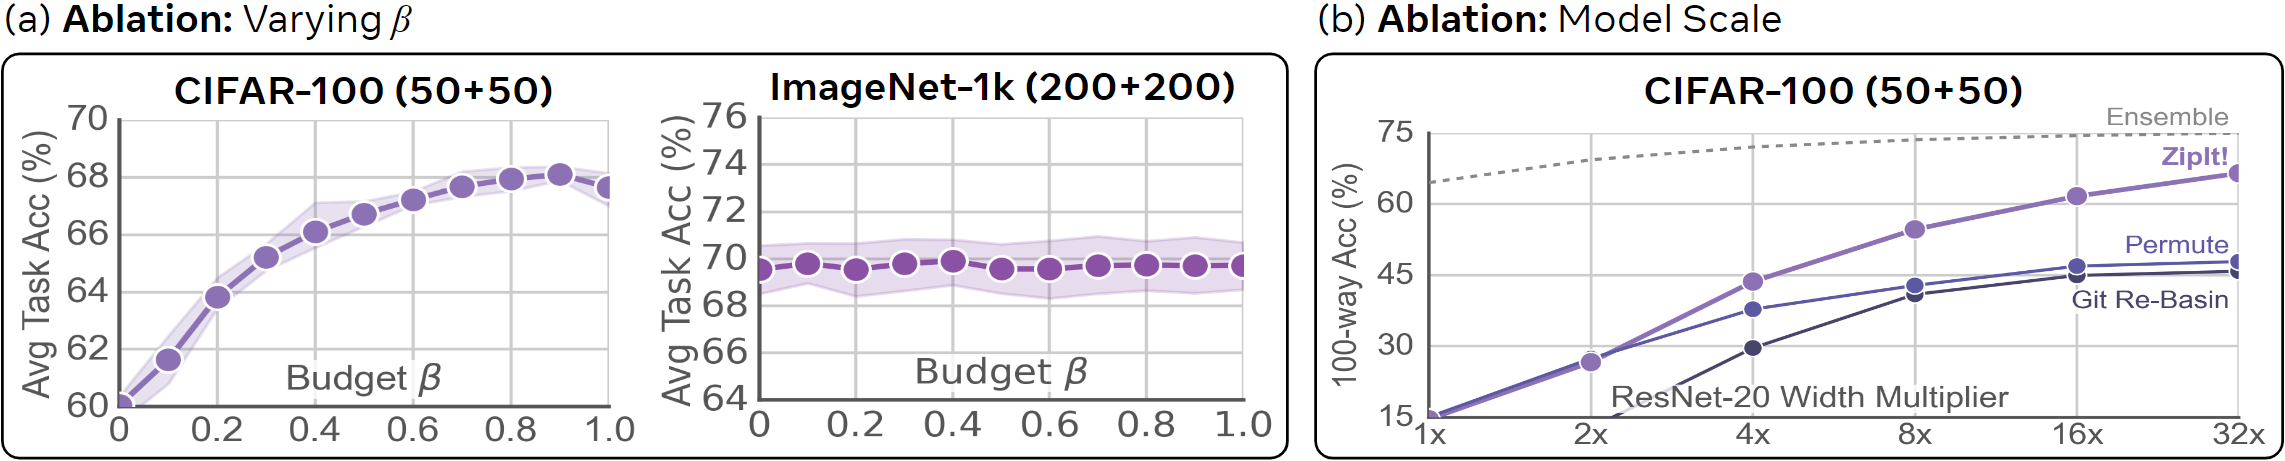
\includegraphics[width=\linewidth]{figures/imgs/varying_beta_and_scale.png}
    \caption{{\bf Varying $\beta$ and Model Scale.} 
    Left: 
    % we test the importance of same model matches by varying the budget $\beta$. A budget of 0 means no same-model matches are allowed, while 1 places no restrictions. 
    We find when the model has enough capacity for the task, a high budget (Sec.~\ref{sec:partial_zip}) improves performance. 
    Right: 
    \name{}\ makes effective use of extra model capacity to quickly reach the ensemble on CIFAR-100 (50+50) when we increase the width of ResNet-20 models. 
    In contrast, our baselines only slightly benefit from the extra scale.
    % Git Re-Basin \cite{ainsworth2022git} and Permute only slightly benefit from the extra scale.
% Git Re-Basin \cite{ainsworth2022git} and Permute only slightly benefit from the extra scale.
    }
    \label{fig:variations}
    % \vspace{-10pt}
\end{figure}

% \begin{figure}
%     \centering
%     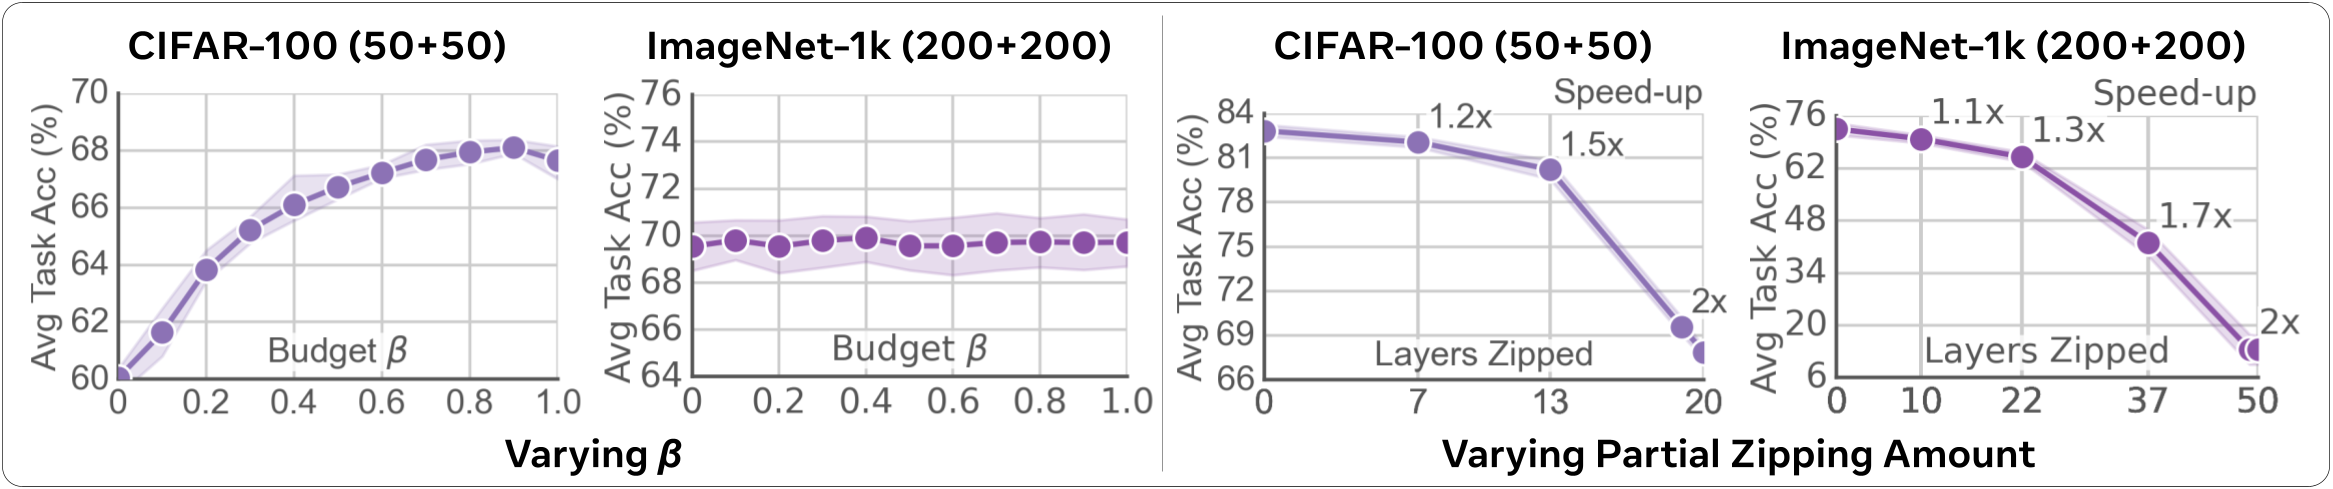
\includegraphics[width=\linewidth]{figures/imgs/zipit_varying_ablations.png}
%     \caption{{\bf Varying $\beta$ and Partial Zipping} (Sec.~\ref{sec:partial_zip}). Left: we test the importance of same model matches by varying the budget $\beta$. A budget of 0 means no same-model matches are allowed, while 1 places no restrictions. We find when the model has enough capacity for the task, a high budget improves performance. Right: by leaving some layers unzipped, we can recover a significant amount of performance while still merging most of the model. 
%     }
%     \label{fig:variations}
% \end{figure}


% \begin{figure}
%     \begin{minipage}[t]{0.48\linewidth}
%         \centering
%         \subfloat[
%             \textbf{CIFAR-100 50+50.}
%             \label{fig:budget_ablation_cifar100}
%         ]{
%             \centering
%             \begin{minipage}{0.48\linewidth}{
%                 \centering
%                 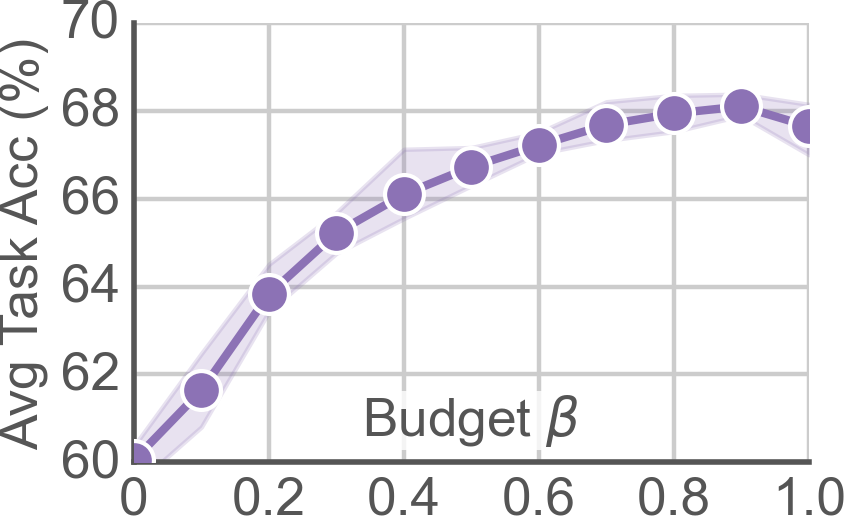
\includegraphics[width=\linewidth]{figures/imgs/cifar100_budget.png}
%             }\end{minipage}
%         }
%         \subfloat[
%             \textbf{ImageNet-1k 200+200.}
%             \label{fig:budget_ablation_imagenet}
%         ]{
%             \centering
%             \begin{minipage}{0.48\linewidth}{
%                 \centering
%                 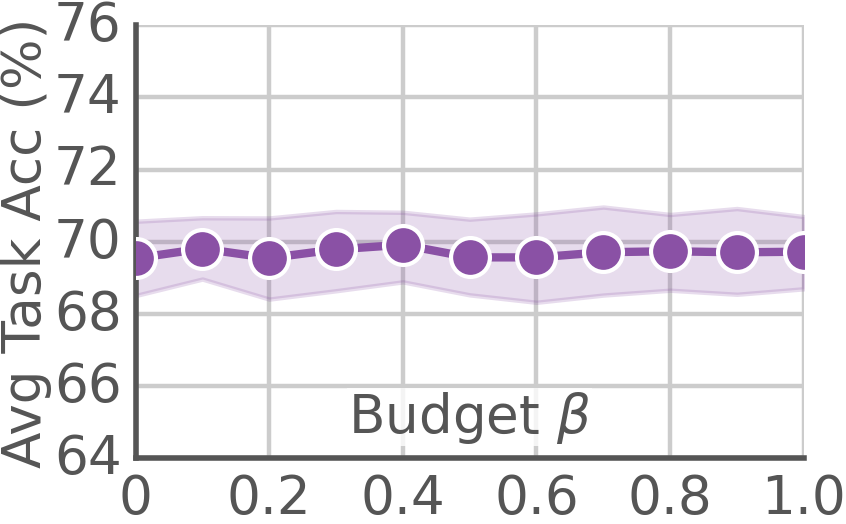
\includegraphics[width=\linewidth]{figures/imgs/imnet_budget.png}
%             }\end{minipage}
%         }
%         \caption{{\bf Varying $\beta$.} We test the importance of same model matches by varying the budget $\beta$ (Sec.~\ref{sec:partial_zip}). A budget of 0 means no same-model matches are allowed, while 1 places no restrictions. We find when the model has enough capacity for the task, a high budget improves performance. }
%         \label{fig:budget_ablation}
%         % \vspace{-80pt}
%     \end{minipage}
%     \hspace{1pt}
%     % \vspace{1em} % Add vertical space between the images
%     \begin{minipage}[t]{0.48\linewidth}
%         \centering
%         \subfloat[
%             \textbf{CIFAR-100 50+50.}
%             \label{fig:partial_zip_cifar100}
%         ]{
%             \centering
%             \begin{minipage}{0.49\linewidth}{
%                 \centering
%                 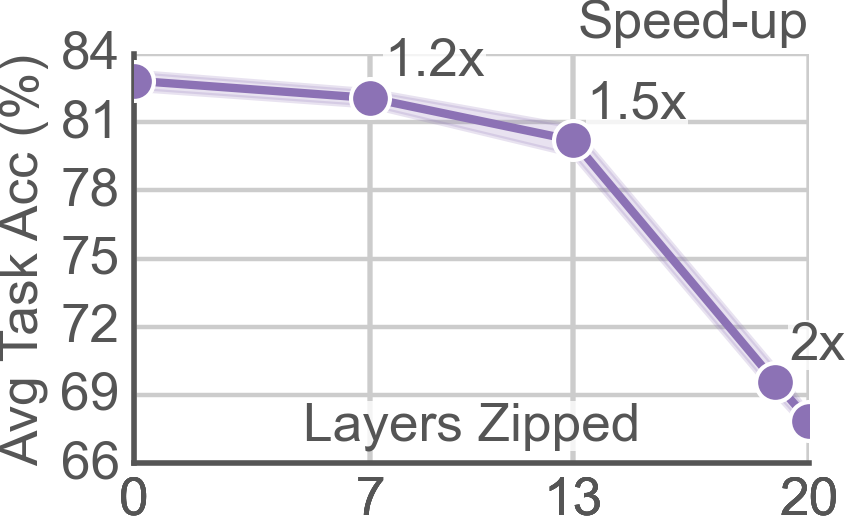
\includegraphics[width=\linewidth]{figures/imgs/partial_zip_CIFAR_50_50.png}
%             }\end{minipage}
%         }
%         \subfloat[
%             \textbf{ImageNet-1k 200+200.}
%             \label{fig:partial_zip_imagenet}
%         ]{
%             \centering
%             \begin{minipage}{0.49\linewidth}{
%                 \centering
%                 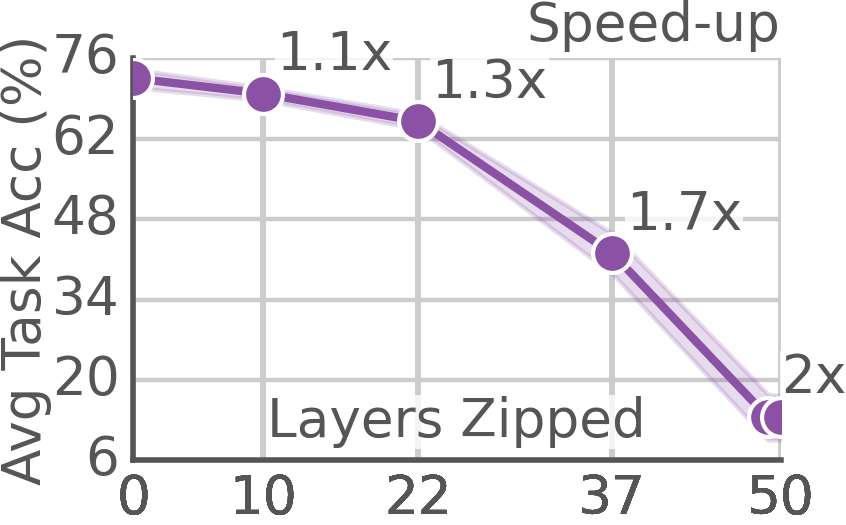
\includegraphics[width=\linewidth]{figures/imgs/partial_zip_imnet_200_200.png}
%             }\end{minipage}
%         }
%         \caption{
%         {\bf Varying Partial Zip.} 
%         By leaving some layers unzipped (Sec.~\ref{sec:partial_zip}), we can recover a significant amount of performance while still merging most of the model. 
%         }
%         \label{fig:varying_partial_zip}
%         % \vspace{10pt}
%     \end{minipage}
%     % \caption{Overall caption for the three images}
%     \vspace{-20pt}
% \end{figure}


%###################



% \begin{figure}[t]
% \centering

% \subfloat[
%     \textbf{CIFAR-100 50+50.}
%     \label{fig:budget_ablation_cifar100}
% ]{
% \centering
% \begin{minipage}{0.48\linewidth}{
% \begin{center}
%     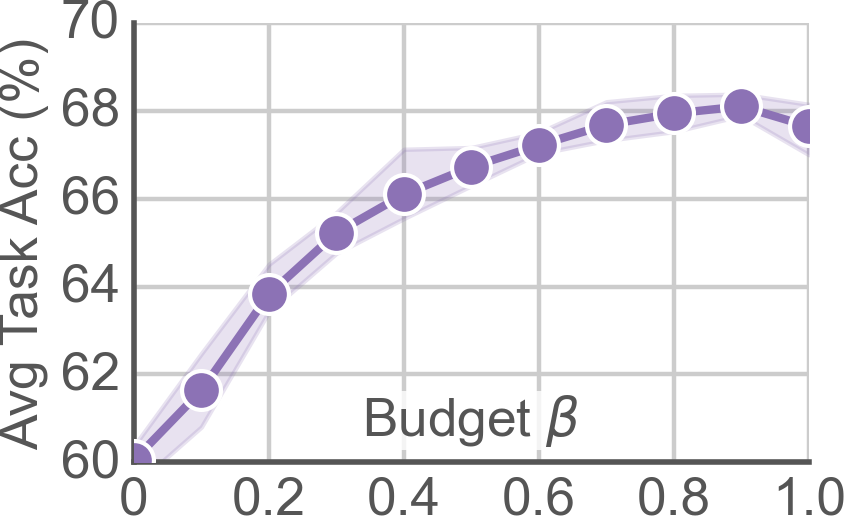
\includegraphics[width=\linewidth]{figures/imgs/cifar100_budget.png}
% \end{center}
% }\end{minipage}
% }
% \subfloat[
%     \textbf{ImageNet-1k 200+200.}
%     \label{fig:budget_ablation_imagenet}
% ]{
% \centering
% \begin{minipage}{0.48\linewidth}{
% \begin{center}
%     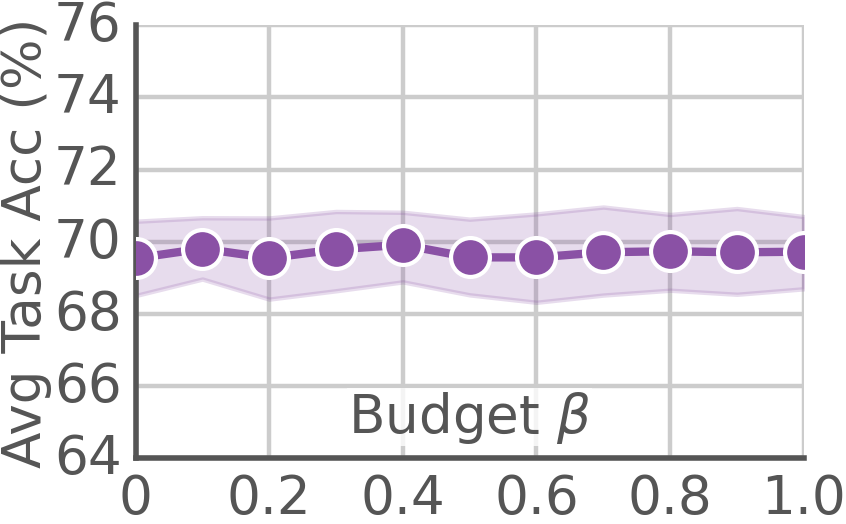
\includegraphics[width=\linewidth]{figures/imgs/imnet_budget.png}
% \end{center}
% }\end{minipage}
% }

% \caption{{\bf Varying $\beta$.} We test the importance of same model matches by varying the budget $\beta$ (Sec.~\ref{sec:partial_zip}). A budget of 0 means no same-model matches are allowed, while 1 places no restrictions. We find when the model has enough capacity for the task, a high budget improves performance. }
% \label{fig:budget_ablation}
% \end{figure}




% \begin{figure}[t]
% \centering

% \subfloat[
%     \textbf{CIFAR-100 50+50.}
%     \label{fig:partial_zip_cifar100}
% ]{
% \centering
% \begin{minipage}{0.49\linewidth}{
% \begin{center}
%     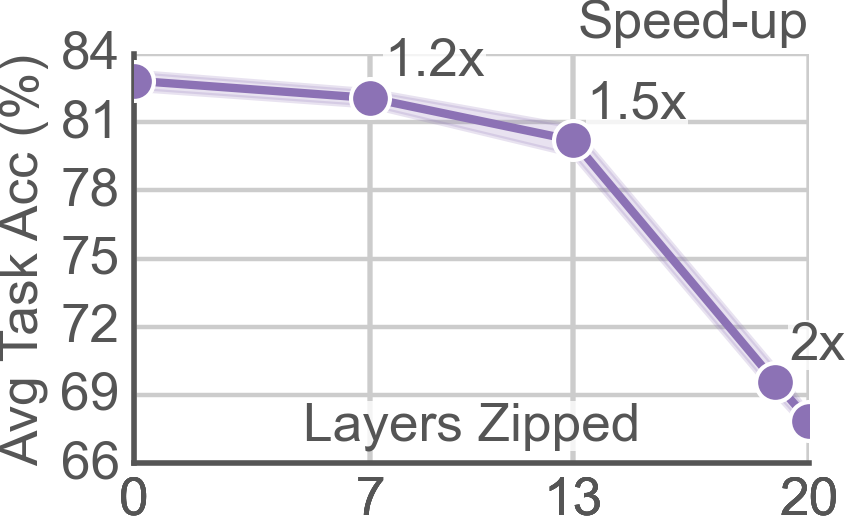
\includegraphics[width=\linewidth]{figures/imgs/partial_zip_CIFAR_50_50.png}
% \end{center}
% }\end{minipage}
% }
% \subfloat[
%     \textbf{ImageNet-1k 200+200.}
%     \label{fig:partial_zip_imagenet}
% ]{
% \centering
% \begin{minipage}{0.49\linewidth}{
% \begin{center}
%     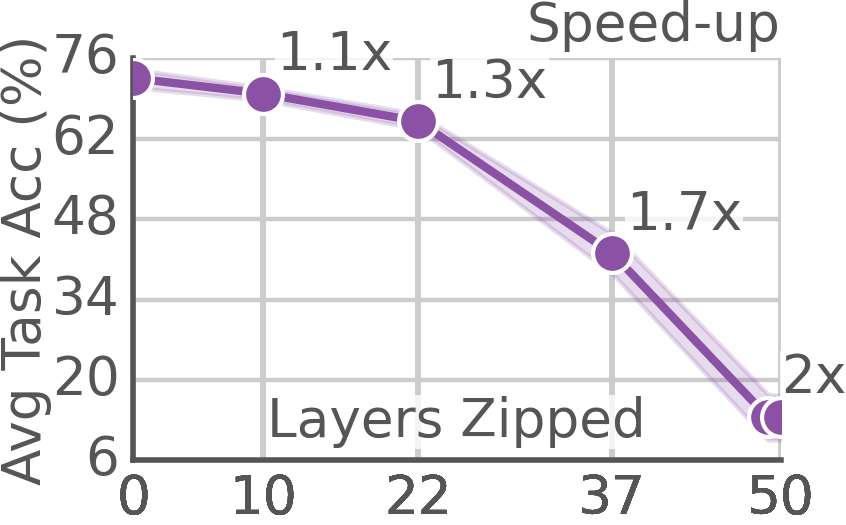
\includegraphics[width=\linewidth]{figures/imgs/partial_zip_imnet_200_200.png}
% \end{center}
% }\end{minipage}
% }

% \caption{
% {\bf Varying Partial Zip.} 
% By leaving some layers unzipped (Sec.~\ref{sec:partial_zip}), we can recover a significant amount of performance while still merging most of the model. 
% }
% \label{fig:varying_partial_zip}
% \end{figure}




% \begin{figure}[t]
% \centering
% %
% \begin{center}
%     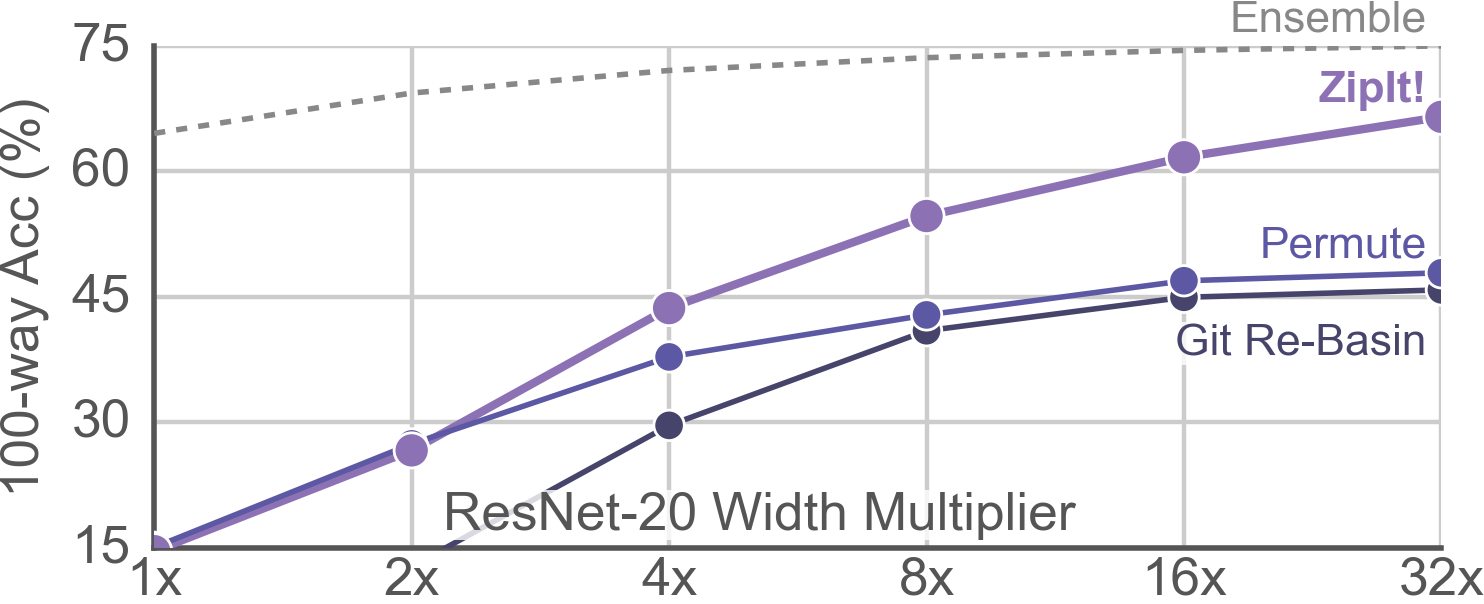
\includegraphics[width=0.95\linewidth]{figures/imgs/model_scale.png}
% \end{center}
% \caption{{\bf Model Scale.} As we increase the width of the ResNet-20 models used for the CIFAR-100 (50+50) setting, \name{}\ makes effective use of that extra capacity, quickly approaching ensemble accuracy. 
% Git Re-Basin \cite{ainsworth2022git} and Permute only slightly benefit from the extra scale.
% }
% \label{fig:model_size}
% \end{figure}


\section{Analysis} \label{sec:ablations}
% Here, we analyze and ablate the performance of \name{}\ on the settings described in Sec.~\ref{sec:results}.


\paragraph{Merging \textit{within} Models.}
A critical piece of \name{}\ compared to prior work is the ability to merge \textit{within} models, not just \textit{across} models. In Sec.~\ref{sec:partial_zip}, we introduce a budget parameter $\beta$ to limit the number of same-model merges, 
and here use CIFAR-100 (50+50) and ImageNet-1k (200+200) to illustrate its effectiveness (Fig.~\ref{fig:variations}\hyperref[fig:variations]{a}).
On CIFAR, same-model merges are very important, with the optimal budget being above 0.8, meaning 80\% of merges are allowed to be within the same model. This is not the case, however, on ImageNet, where the difficulty of the task means there likely are much fewer redundant features \textit{within} each model.

\paragraph{Model Scale.}
In Fig.~\ref{fig:variations}\hyperref[fig:variations]{b}, we test the effect of model scale directly by evaluating joint accuracy on our CIFAR-100 (50+50) setting with ResNet-20 models of increasing width. Here, we explicitly see that when the width of the models are too small for the task (e.g., $<4\times$), \name{}\ and the Permute baseline perform identically (though both much better than Git Re-Basin). However, when the scale increases, \name{}\ trends toward the ensemble upper bound of 75\%, while both the Permute baseline and Git Re-Basin plateau at around 45\%. This corroborates Eq.~\ref{eq:mainpaper_barrier} and indicates our method uses the extra model capacity effectively, much better than prior work.
\begin{wrapfigure}{r}{0.5\textwidth}
% \vspace{-10pt}
\resizebox{0.48\textwidth}{!}{
        \tablestyle{7pt}{1.05}
        \begin{tabular}{y{55}x{43}x{22}x{30}}
            Algorithm & \modela{A}$\leftrightarrow$\modela{A}/\modelb{B}$\leftrightarrow$\modelb{B}? & Acc & Time\\
            \shline
            Identity {\scriptsize (Eq.~\ref{eq:wavg})}                  & \xmark{} & {43.0\conf{3.1}} & {1.8\unit{ms}} \\
            Permute {\scriptsize (Eq.~\ref{eq:rebasin})}                & \xmark{} & {58.4\conf{1.3}} & {28\unit{ms}} \\
            K-Means                                                     & \checkmark{} & {29.1\conf{5.5}} & {19\unit{sec}} \\
            \hline
            \multicolumn{4}{c}{Zip {\scriptsize (Eq.~\ref{eq:zip})}} \\
            Optimal Match                                               & \checkmark{} & {\bf 79.6\conf{1.7}} & {11\unit{min}} \\
            Greedy Match                                                & \checkmark{} & {\bf 79.0\conf{1.8}} & {1.1\unit{sec}} \\
            Greedy, $\alpha$=0.1 & \default{\checkmark{}} & \default{\textbf{79.1\conf{2.1}}}  &  \default{1.2\unit{sec}}  \\
        \end{tabular}
    }
    \captionof{table}{{\bf Comparing Matching Algorithms} to use for \modelc{$M_i$} on CIFAR-10 (5+5) joint 10-way accuracy.
    Permuting \modelb{B}$\rightarrow$\modela{A} as in prior work (Eq.~\ref{eq:rebasin}) performs poorly. 
    We significantly improve by merging features \textit{within} each model (Eq.~\ref{eq:zip}).
    Our greedy approach is nearly as accurate as the optimal algorithm while being two orders of magnitude faster. 
    }
    \label{tab:matching_alg}
    \vspace{-10pt}
\end{wrapfigure}
% \end{table}


% \begin{wrapfigure}{l}{0.48\linewidth}
% % \vspace{-260pt}
% \begin{minipage}[l]{\linewidth}{
%     \begin{minipage}[c]{\linewidth}
%         \centering
%         \resizebox{\textwidth}{!}{
%             \tablestyle{7pt}{1.05}
%             \begin{tabular}{y{55}x{43}x{22}x{30}}
%                 Algorithm & \modela{A}$\leftrightarrow$\modela{A}/\modelb{B}$\leftrightarrow$\modelb{B}? & Acc & Time\\
%                 \shline
%                 Identity {\scriptsize (Eq.~\ref{eq:wavg})}                  & \xmark{} & {43.0\conf{3.1}} & {1.8\unit{ms}} \\
%                 Permute {\scriptsize (Eq.~\ref{eq:rebasin})}                & \xmark{} & {58.4\conf{1.3}} & {28\unit{ms}} \\
%                 K-Means                                                     & \checkmark{} & {29.1\conf{5.5}} & {19\unit{sec}} \\
%                 \hline
%                 \multicolumn{4}{c}{Zip {\scriptsize (Eq.~\ref{eq:zip})}} \\
%                 Optimal Match                                               & \checkmark{} & {\bf 79.6\conf{1.7}} & {11\unit{min}} \\
%                 Greedy Match                                                & \checkmark{} & {\bf 79.0\conf{1.8}} & {1.1\unit{sec}} \\
%                 Greedy, $\alpha$=0.1 & \default{\checkmark{}} & \default{\textbf{79.1\conf{2.1}}}  &  \default{1.2\unit{sec}}  \\
%             \end{tabular}
%         }
%         \captionof{table}{{\bf Matching Algorithm} to use for \modelc{$M_i$}. 
%         Permuting \modelb{B}$\rightarrow$\modela{A} as in prior work (Eq.~\ref{eq:rebasin}) performs poorly, thus we allow merging features \textit{within} each model (Eq.~\ref{eq:zip}).
%         Our greedy approach is nearly as accurate as the optimal algorithm while being two orders of magnitude faster. 
%         ``Acc'' is CIFAR-10 (5+5) joint 10-way accuracy.
%         }
%         \label{tab:matching_alg}
%     \end{minipage}
%     \vspace{10pt}
%     \begin{minipage}[c]{\linewidth}
%         % \vspace{40pt}
%         \centering
%         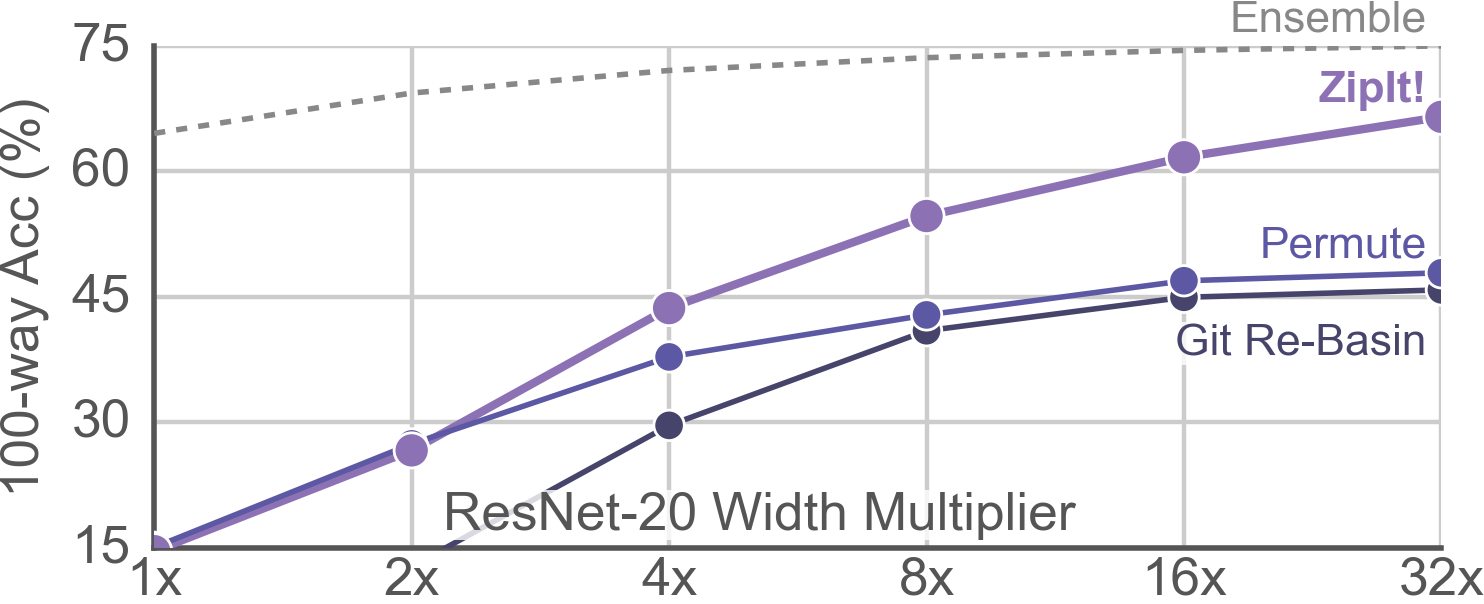
\includegraphics[width=0.95\linewidth]{figures/imgs/model_scale.png}
%         \caption{{\bf Model Scale.} 
%         \name{}\ makes effective use of extra model capacity to quickly reach the ensemble on CIFAR-100 (50+50) when we increase the width of ResNet-20 models.
%         % \name{}\ quickly approaches ensemble accuracy as we increase the width of the ResNet-20 models in the CIFAR-100 (50+50) setting, making effective use of extra capacity from scale.
%         % As we increase the width of the ResNet-20 models used for the CIFAR-100 (50+50) setting, \name{}\ makes effective use of that extra capacity, quickly approaching ensemble accuracy. 
%         Git Re-Basin \cite{ainsworth2022git} and Permute only slightly benefit from the extra scale.
%         }
%         \label{fig:model_size}
%         \vspace{-30pt}
%     \end{minipage}
% }\end{minipage}
% \end{wrapfigure}










% \begin{table}[t]
% \centering

% \tablestyle{7pt}{1.05}
% \begin{tabular}{y{50}x{43}x{22}x{30}}
%     Algorithm & \modela{A}$\leftrightarrow$\modela{A}/\modelb{B}$\leftrightarrow$\modelb{B}? & Acc & Time\\
%     \shline
%     Identity {\scriptsize (Eq.~\ref{eq:wavg})}                  & \xmark{} & {43.0\conf{3.1}} & {1.8\unit{ms}} \\
%     Permute {\scriptsize (Eq.~\ref{eq:rebasin})}                & \xmark{} & {58.4\conf{1.3}} & {28\unit{ms}} \\
%     K-Means                                                     & \checkmark{} & {29.1\conf{5.5}} & {19\unit{sec}} \\
%     \hline
%     \multicolumn{4}{c}{Zip {\scriptsize (Eq.~\ref{eq:zip})}} \\
%     Optimal Match                                               & \checkmark{} & {\bf 79.6\conf{1.7}} & {11\unit{min}} \\
%     Greedy Match                                                & \checkmark{} & {\bf 79.0\conf{1.8}} & {1.1\unit{sec}} \\
%     Greedy, $\alpha$=0.1 & \default{\checkmark{}} & \default{\textbf{79.1\conf{2.1}}}  &  \default{1.2\unit{sec}}  \\
% \end{tabular}
% \caption{{\bf Matching Algorithm} to use for \modelc{$M_i$}. 
% Permuting \modelb{B}$\rightarrow$\modela{A} as in prior work (Eq.~\ref{eq:rebasin}) performs poorly, thus we allow merging features \textit{within} each model (Eq.~\ref{eq:zip}).
% Our greedy approach is nearly as accurate as the optimal algorithm while being two orders of magnitude faster. 
% ``Acc'' is CIFAR-10 (5+5) joint 10-way accuracy.
% }
% \label{tab:matching_alg}
% \end{table}

\vspace{-1em}
\paragraph{Matching Algorithm.}
In Tab.~\ref{tab:matching_alg}, we compare matching algorithms used to compute \modelc{$M_i$} in Eq.~\ref{eq:zip}. Using either the identity (weight averaging) or a permutation (as in prior work) underperforms on CIFAR-10 (5+5) joint 10-way classification. 
In contrast, we obtain up to 21.2\% higher accuracy if we allow both permutations and \textit{merging within models}.
% In contrast, if we allow merging \textit{within} models as well, then we obtain up to 21.2\% higher accuracy than permuting alone. 
However, doing this optimally is difficult, as the standard linear sum assignment algorithm assumes bipartite matches. We could use a optimal graph-based solver (e.g., \citet{networkx}) instead, but doing so is prohibitively slow (11 minutes to transform a ResNet-20$\times$4 model). Thus, we find matches greedily by repeatedly taking the most correlated pair of features without replacement. This performs almost as well, and is multiple orders of magnitude faster. If we allow repeated matches (Sec.~\ref{sec:partial_zip}), we obtain a slightly better result.
Like \citet{bolya2022token}, we find that matching is better for merging features than clustering (K-Means).

% % \begin{wrapfigure}{l}{0.48\linewidth}
% % \begin{figure}[t]
% \centering
% %
% \begin{center}
%     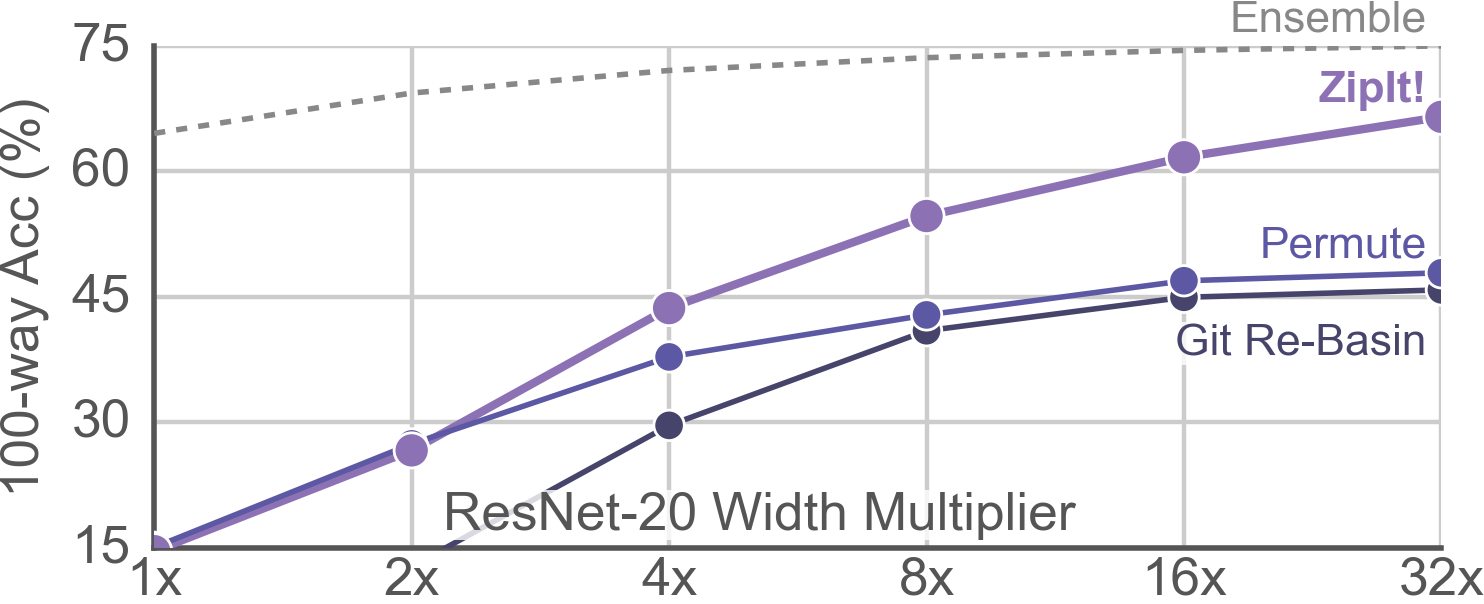
\includegraphics[width=0.95\linewidth]{figures/imgs/model_scale.png}
% \end{center}
% \caption{{\bf Model Scale.} As we increase the width of the ResNet-20 models used for the CIFAR-100 (50+50) setting, \name{}\ makes effective use of that extra capacity, quickly approaching ensemble accuracy. 
% Git Re-Basin \cite{ainsworth2022git} and Permute only slightly benefit from the extra scale.
% }
% \label{fig:model_size}
% \end{wrapfigure}
% % \end{figure}
% indicates that our method uses the extra capacity of these models effectively, much better than prior work.

% % \begin{figure}[t]
% \centering

% \subfloat[
%     \textbf{CIFAR-100 50+50.}
%     \label{fig:partial_zip_cifar100}
% ]{
% \centering
% \begin{minipage}{0.49\linewidth}{
% \begin{center}
%     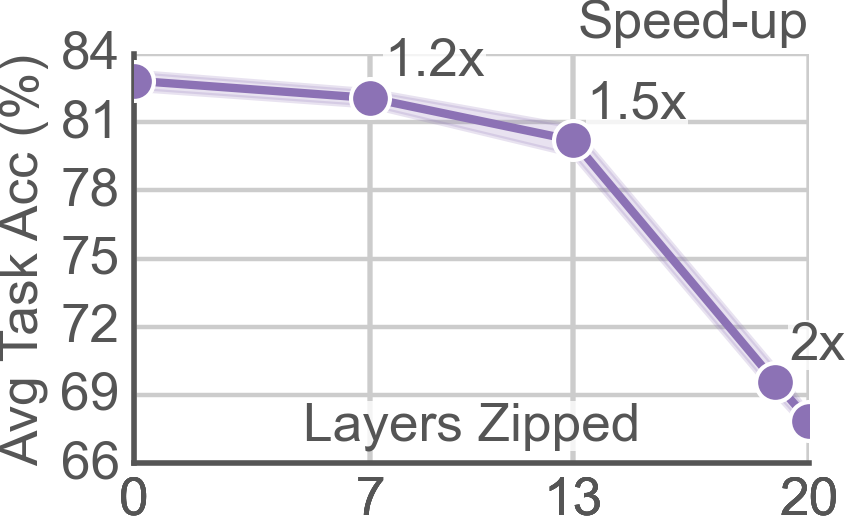
\includegraphics[width=\linewidth]{figures/imgs/partial_zip_CIFAR_50_50.png}
% \end{center}
% }\end{minipage}
% }
% \subfloat[
%     \textbf{ImageNet-1k 200+200.}
%     \label{fig:partial_zip_imagenet}
% ]{
% \centering
% \begin{minipage}{0.49\linewidth}{
% \begin{center}
%     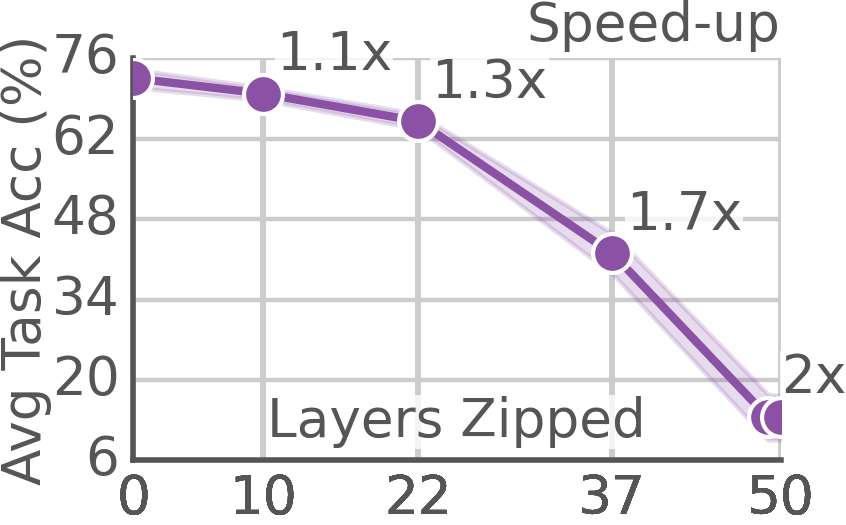
\includegraphics[width=\linewidth]{figures/imgs/partial_zip_imnet_200_200.png}
% \end{center}
% }\end{minipage}
% }

% \caption{
% {\bf Varying Partial Zip.} 
% By leaving some layers unzipped (Sec.~\ref{sec:partial_zip}), we can recover a significant amount of performance while still merging most of the model. 
% }
% \label{fig:varying_partial_zip}
% \end{figure}

% \begin{wrapfigure}{r}{0.48\linewidth}
% \vspace{-10pt}
% \centering
% \resizebox{\linewidth}{!}{
%     \tablestyle{5pt}{1.1}
%     {
%     \tablestyle{5pt}{1.1}
%     \begin{tabular}{x{40}x{40}x{40}}
%         \multicolumn{3}{c}{Average Stage Correlations}\\
%         Layer \sfrac{7}{20} & Layer \sfrac{13}{20} & Layer \sfrac{19}{20}\\
%     \shline
%     {0.50\conf{0.01}} & {0.37\conf{0.00}} & {0.27\conf{0.00}} \\
%     \hline
% \end{tabular}
%     }
% }
% \captionof{table}{\textbf{CIFAR-100 (50+50) Zipping Correlations.} We show the average correlations between two ResNet-20 ($8\times$) models at each partial zipping stage. Correlations consistently decrease at each successive stage, indicating that the layers of the two models increasingly diverge. 
% }
% \label{tab:partialzip_corrs}
% % \end{table}
% \vspace{-20pt}
% \end{wrapfigure}


\begin{wrapfigure}{r}{0.48\linewidth}
\vspace{-15pt}
\begin{minipage}[l]{\linewidth}{
\captionsetup{justification=centering}
\subfloat[
    \textbf{CIFAR-100 \\ \ \ \ \ (50+50)}
    \label{fig:partial_zip_cifar100}
]{
\centering
\begin{minipage}{0.48\linewidth}{
\begin{center}
    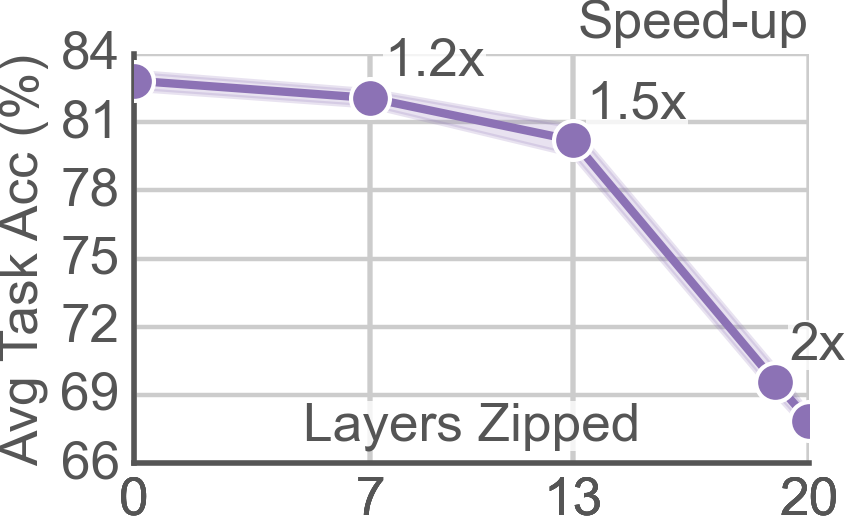
\includegraphics[width=\linewidth]{figures/imgs/partial_zip_CIFAR_50_50.png}
\end{center}
}\end{minipage}
}
\subfloat[
    \textbf{ImageNet-1k \\ \ \ \  (200+200)}
    \label{fig:partial_zip_imagenet}
]{
\centering
\begin{minipage}{0.48\linewidth}{
\begin{center}
    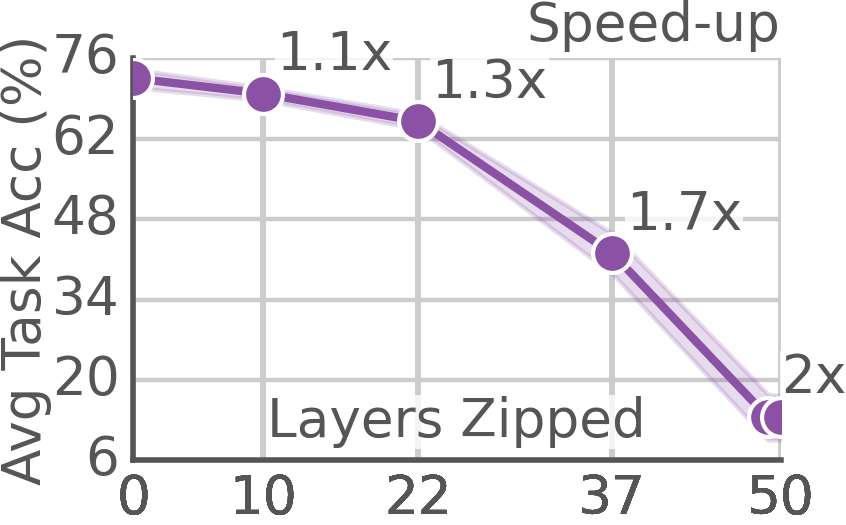
\includegraphics[width=\linewidth]{figures/imgs/partial_zip_imnet_200_200.png}
\end{center}
}\end{minipage}
}
\captionsetup{justification=justified}
        \caption{{\bf Varying Partial Zip.} By leaving some layers unzipped (Sec.~\ref{sec:partial_zip}), we can recover a significant amount of performance while still merging most of the model. }
\label{fig:varying_partial_zip}
}\end{minipage}
\begin{minipage}[l]{\linewidth}{
\vspace{5pt}
\centering
\resizebox{\linewidth}{!}{
    \tablestyle{5pt}{1.1}
    {
    \tablestyle{5pt}{1.1}
    \begin{tabular}{x{40}x{40}x{40}}
        \multicolumn{3}{c}{Average Stage Correlations}\\
        Layer \sfrac{7}{20} & Layer \sfrac{13}{20} & Layer \sfrac{19}{20}\\
    \shline
    {0.50\conf{0.01}} & {0.37\conf{0.00}} & {0.27\conf{0.00}} \\
    \hline
\end{tabular}
    }
}
\captionof{table}{\textbf{CIFAR-100 (50+50) Zipping Correlations.} We show the average correlations between two ResNet-20 ($8\times$ width) models at each partial zipping stage. Correlations consistently decrease at each successive stage, indicating that the layers of the two models increasingly diverge. 
}
\label{tab:partialzip_corrs}
% \end{table}
% \vspace{10pt}
}\end{minipage}
\begin{minipage}[l]{\linewidth}{
\captionsetup{justification=centering}
\vspace{1em}
\subfloat[
    \textbf{CIFAR-100 \\ \ \ \ \ (50+50)}
    \label{fig:data_use_cifar100}
]{
\centering
\begin{minipage}{0.48\linewidth}{
\begin{center}
    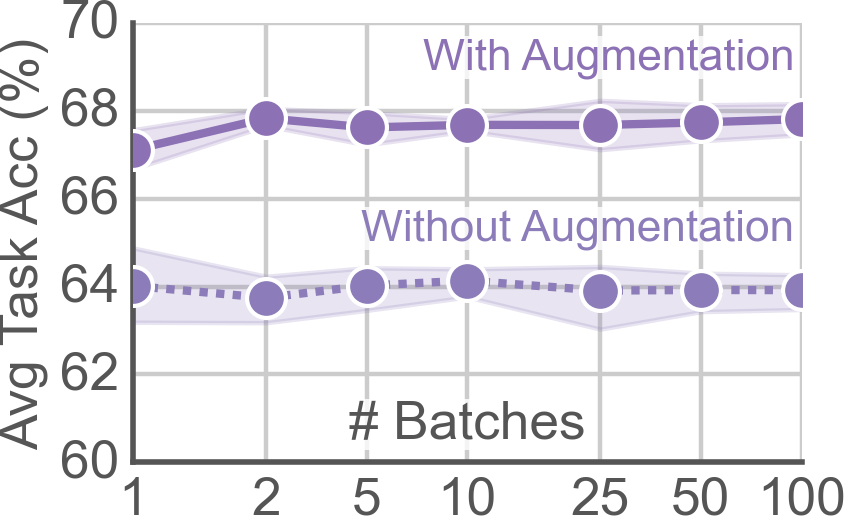
\includegraphics[width=\linewidth]{figures/imgs/cifar100_data.png}
\end{center}
}\end{minipage}
}
\subfloat[
    \textbf{ImageNet-1k \\ \ \ \  (200+200)}
    \label{fig:data_use_imagenet}
]{
\centering
\begin{minipage}{0.48\linewidth}{
\begin{center}
    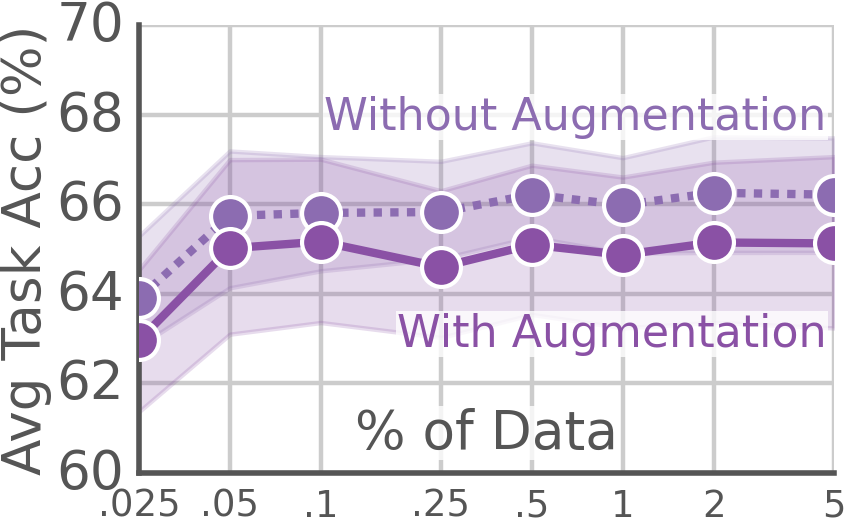
\includegraphics[width=\linewidth]{figures/imgs/imnet200_data.png}
\end{center}
}\end{minipage}
}
\captionsetup{justification=justified}
\caption{
{\bf Data Usage.} 
How much data do we need to use to compute activations? 
We find that only a few hundred images are needed to obtain the best performance.
Data augmentation is not always useful.
% Here we ablate the amount of data used for our CIFAR-100 (50+50) ResNet-20 ($8\times$ width) and ImageNet (200+200) Resnet-50 (\sfrac{22}{50} layers) experiments. 
% The batch size used is 500 for CIFAR and 16 for ImageNet. 
% In both cases, we only need a few hundred images to obtain the best results. 
% On the other hand, data augmentation is necessary for CIFAR but hurts for ImageNet. Our default for all experiments uses data augmentation and the full set for CIFAR (100 batches) and 1\% of the data for ImageNet. 
}
\label{fig:data_usage}
}\end{minipage}
% \vspace{-60pt}
\end{wrapfigure}

% \begin{wrapfigure}{l}{0.52\linewidth}
% % \vspace{-260pt}
% \begin{minipage}[l]{\linewidth}{
% \subfloat[
%     \textbf{CIFAR-100 (50+50).}
%     \label{fig:data_use_cifar100}
% ]{
% \centering
% \begin{minipage}{0.48\linewidth}{
% \begin{center}
%     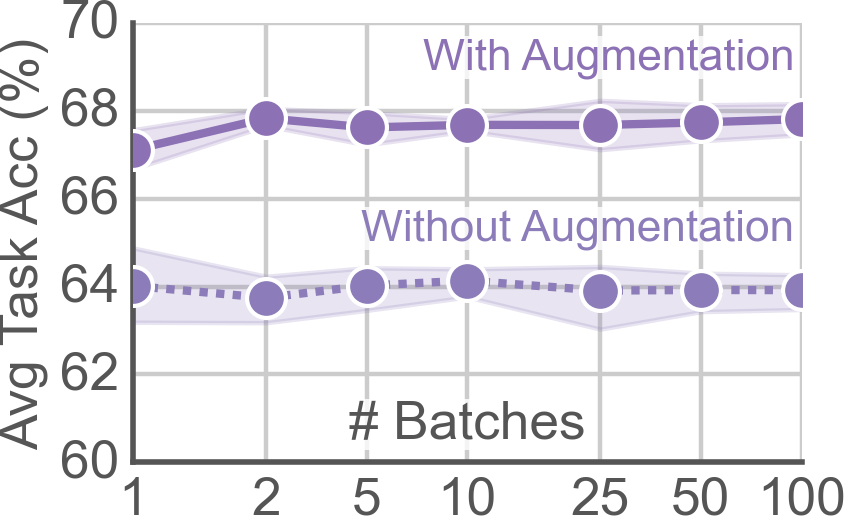
\includegraphics[width=\linewidth]{figures/imgs/cifar100_data.png}
% \end{center}
% }\end{minipage}
% }
% \subfloat[
%     \textbf{ImageNet-1k (200+200).}
%     \label{fig:data_use_imagenet}
% ]{
% \centering
% \begin{minipage}{0.48\linewidth}{
% \begin{center}
%     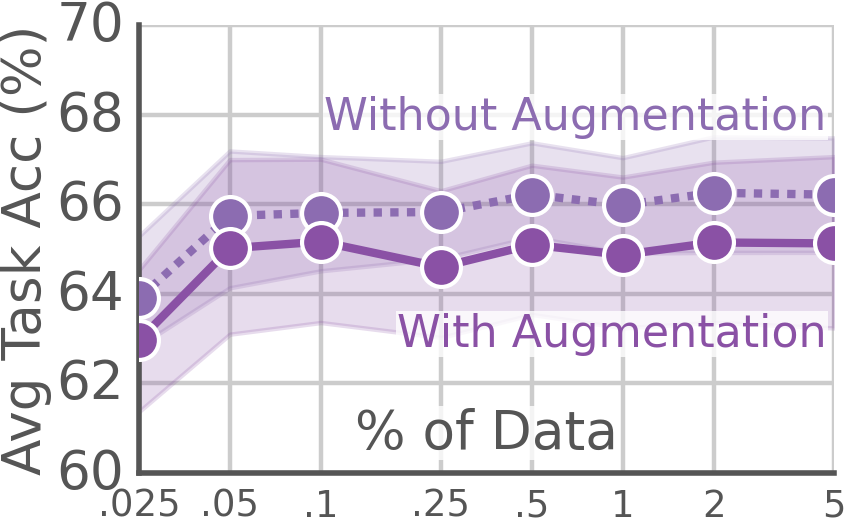
\includegraphics[width=\linewidth]{figures/imgs/imnet200_data.png}
% \end{center}
% }\end{minipage}
% }
%         \caption{
%         {\bf Data Usage.} How much data do we need to use to compute activations? Here we ablate the amount of data used for our CIFAR-100 (50+50) ResNet-20 ($8\times$ width) and ImageNet (200+200) Resnet-50 (\sfrac{22}{50} layers) experiments. The batch size used is 500 for CIFAR and 16 for ImageNet. In both cases, we only need a few hundred images to obtain the best results. On the other hand, data augmentation is necessary for CIFAR but hurts for ImageNet. Our default for all experiments uses data augmentation and the full set for CIFAR (100 batches) and 1\% of the data for ImageNet. 
%         }
% \label{fig:data_usage}
% }\end{minipage}
% \end{wrapfigure}


% \caption{{\bf Data Usage.} How much data do we need to use to compute activations? Here we ablate the amount of data used for our CIFAR-100 (50+50) ResNet-20 ($8\times$ width) and ImageNet (200+200) Resnet-50 (\sfrac{22}{50} layers) experiments. The batch size used is 500 for CIFAR and 16 for ImageNet. In both cases, we only need a few hundred images to obtain the best results. On the other hand, data augmentation is necessary for CIFAR but hurts for ImageNet. Our default for all experiments uses data augmentation and the full set for CIFAR (100 batches) and 1\% of the data for ImageNet. }
% \label{fig:data_usage}
% \end{figure}


% \begin{figure}
%     \begin{minipage}[t]{0.50\linewidth}
%         \centering
%         \subfloat[
%             \textbf{CIFAR-100 (50+50).}
%             \label{fig:partial_zip_cifar100}
%         ]{
%             \centering
%             \begin{minipage}{0.40\linewidth}{
%                 \centering
%                 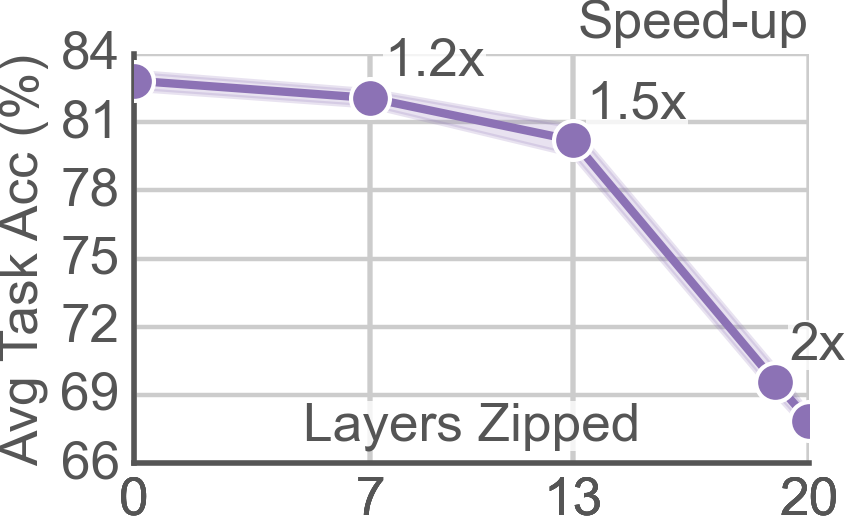
\includegraphics[width=\linewidth]{figures/imgs/partial_zip_CIFAR_50_50.png}
%             }\end{minipage}
%         }
%         \subfloat[
%             \textbf{ImageNet-1k (200+200).}
%             \label{fig:partial_zip_imagenet}
%         ]{
%             \centering
%             \begin{minipage}{0.40\linewidth}{
%                 \centering
%                 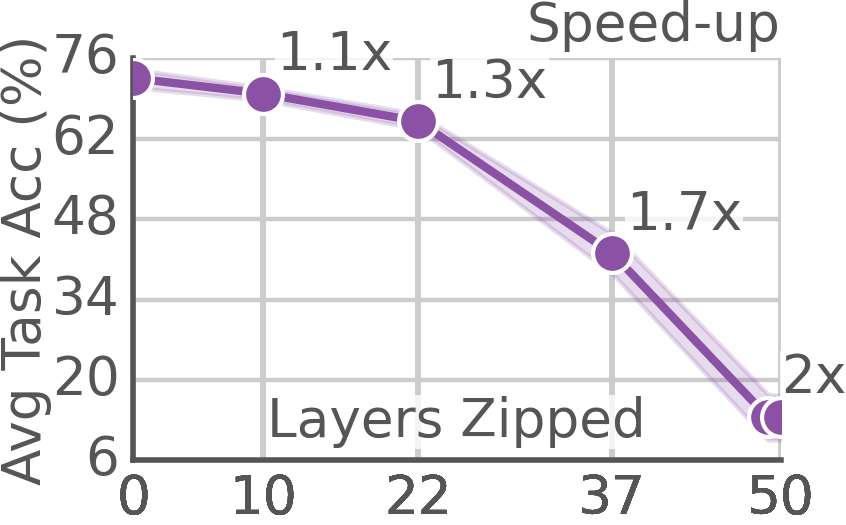
\includegraphics[width=\linewidth]{figures/imgs/partial_zip_imnet_200_200.png}
%             }\end{minipage}
%         }
%         \caption{{\bf Varying Partial Zip.} 
%             By leaving some layers unzipped (Sec.~\ref{sec:partial_zip}), we can recover a significant amount of performance while still merging most of the model.  }
%         \label{fig:varying_partial_zip}
%         % \vspace{-80pt}
%     \end{minipage}
%     \hspace{1pt}
%     % \vspace{1em} % Add vertical space between the images
%     \begin{minipage}[t]{0.48\linewidth}
%         \centering
%         \subfloat[
%             \textbf{CIFAR-100 (50+50).}
%             \label{fig:data_use_cifar100}
%         ]{
%             \centering
%             \begin{minipage}{0.48\linewidth}{
%                 \centering
%                 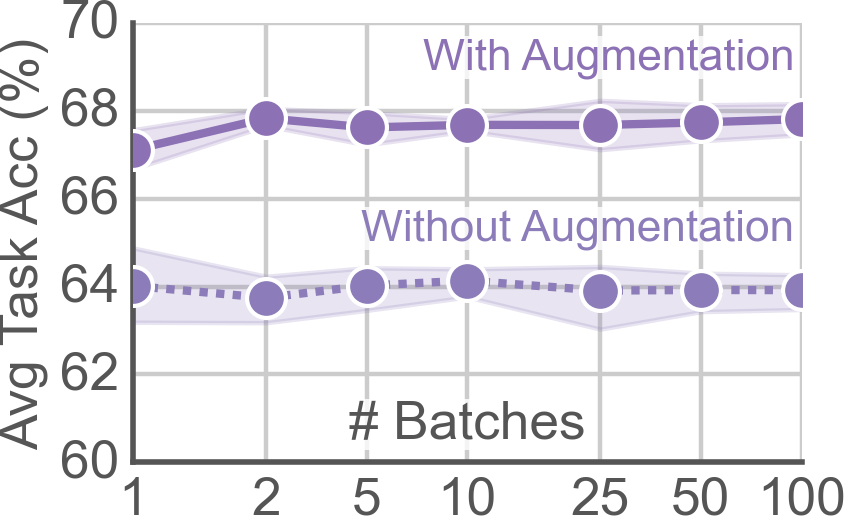
\includegraphics[width=\linewidth]{figures/imgs/cifar100_data.png}
%             }\end{minipage}
%         }
%         \subfloat[
%             \textbf{ImageNet-1k (200+200).}
%             \label{fig:data_use_imagenet}
%         ]{
%             \centering
%             \begin{minipage}{0.48\linewidth}{
%                 \centering
%                 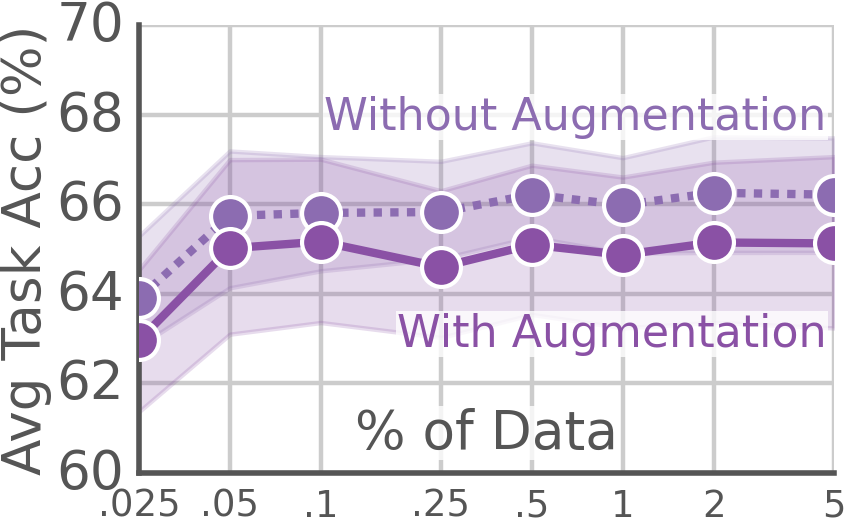
\includegraphics[width=\linewidth]{figures/imgs/imnet200_data.png}
%             }\end{minipage}
%         }
%         \caption{
%         {\bf Data Usage.} How much data do we need to use to compute activations? Here we ablate the amount of data used for our CIFAR-100 (50+50) ResNet-20 ($8\times$ width) and ImageNet (200+200) Resnet-50 (\sfrac{22}{50} layers) experiments. The batch size used is 500 for CIFAR and 16 for ImageNet. In both cases, we only need a few hundred images to obtain the best results. On the other hand, data augmentation is necessary for CIFAR but hurts for ImageNet. Our default for all experiments uses data augmentation and the full set for CIFAR (100 batches) and 1\% of the data for ImageNet. 
%         }
%         \label{fig:data_usage}
%         % \vspace{10pt}
%     \end{minipage}
%     % \caption{Overall caption for the three images}
%     \vspace{-20pt}
% \end{figure}

% \paragraph{Partial Zipping.} Overall, we find partial zipping to be a simple yet effective technique to add capacity back to the merged model. For CIFAR-100, we can obtain near ensemble accuracies at a 1.5$\times$ speed-up (Tab.~\ref{tab:cifar50+50}). Similarly on a difficult setting like ImageNet, partial zipping is \textit{necessary} to obtain any reasonable accuracy. Additional results in Appendix~\ref{ap:partial_zipping}.

% In Fig.~\ref{fig:variations}, we plot the average per task accuracy by the number of layers zipped in ResNet-20$\times$8 for CIFAR-100 (50+50) and ResNet-50 for ImageNet-1k (200+200). Note that to avoid adding extra unmerge modules into the network, our stopping point while unzipping has to be the end of a stage. 
% Overall, we find partial zipping to be a simple yet effective technique to add capacity back to the merged model. For CIFAR-100, we can obtain near ensemble accuracies at a 1.5$\times$ speed-up. Similarly on a difficult setting like ImageNet, partial zipping is \textit{necessary} to obtain any reasonable accuracy.
